%
% I'm adding an outline here so I can see how everything fits together

%
% \title{Exploiting First-Class Arrays in Fortran for Accelerator Programming}
%

%
% \abstract
%

%
% \section{Introduction}
%    \subsection{Approach}
%    \subsection{Why Fortran?}
%    \subsection{Comparison to Other Languages}
%

%
% \section{Programming model}
%    \subsection{Fortran Syntax}   
%       \subsubsection*{Array notation}
%       \subsubsection*{Elemental functions}
%       \subsubsection*{Pure procedures}
%       \subsubsection*{Shift functions}
%       \subsubsection*{Regions}
%    \subsection{New Functions}
%    \subsection{Parallelism}
%    \subsection{Limitations}
%

%
% \section{Shallow Water Model}
%    \subsection{Equations}
%

%
% \section{Source-To-Source Transformations}
%    \subsection{ForOpenCL}
%       \subsubsection{array syntax}
%       \subsubsection{where construct}
%    \subsection{New functions}
%       \subsubsection{region}
%    \subsection{Static Analysis}
%       \subsubsection{Analysis not required}
%    \subsection{Simplifying Assumptions}
%

%
% \section{Performance}
%

%
% \section{Conclusions}
%


\documentclass[10pt, conference, compsocconf]{IEEEtran}

\usepackage{cite}
\usepackage{graphicx}
\usepackage[cmex10]{amsmath}
\usepackage{amssymb}
\usepackage{array}
\usepackage{url}
\usepackage{listings}

\lstdefinestyle{FortranLike}{float,frame=lines,language=Fortran,commentstyle=\ttfamily,basicstyle=\ttfamily}
\lstdefinestyle{CLike}{float,frame=lines,language=C,commentstyle=\ttfamily,basicstyle=\ttfamily}
\lstdefinestyle{NoFloatCLike}{frame=lines,language=C,commentstyle=\ttfamily,basicstyle=\ttfamily}


\title{Exploiting Array Syntax in Fortran for Accelerator Programming}

%%
%% reorder appropriately later
%%
\author{\IEEEauthorblockN{Matthew J. Sottile}
\IEEEauthorblockA{Galois, Inc.\\
%421 SW 6th Ave. Suite 300 \\
%Portland, OR 97204\\
matt@galois.com}
\and
\IEEEauthorblockN{Craig E Rasmussen,\\
                  Wayne N. Weseloh,\\
                  Robert W. Robey}
\IEEEauthorblockA{Los Alamos National Laboratory\\
%CCS-7, MS B287\\
%Los Alamos, NM\\
\{crasmussen, weseloh, brobey\}@lanl.gov}

\and
\IEEEauthorblockN{Daniel Quinlan}
\IEEEauthorblockA{Lawrence Livermore\\ National Laboratory\\
dquinlan@llnl.gov}

\and
\IEEEauthorblockN{Jeffrey Overbey}
\IEEEauthorblockA{Indiana University\\
overbey2@illinois.edu}

}

\begin{document}

\maketitle

\begin{abstract}
Emerging architectures for high performance computing are well suited
to a data-parallel programming model.  This paper presents a simple
programming methodology that allows programmers to take advantage of
these emerging systems.  We use array constructs in Fortran 90 to show how this
infrequently exploited, standardized language feature is easily
transformed to lower-level accelerator code.  These transformations
are based on a simple mapping from Fortran 90 to OpenCL.  We
demonstrate, using a shallow-water code, that an acceleration of up to 40
times can be achieved on GPU hardware with these compiler-generated
transformations.
\end{abstract}

It has been hard historically to create parallel programs.  The responsibility
(and difficulty) of creating \emph{correct} parallel programs can be viewed as
being spread between the programmer and the compiler.
Ideally we would like to have parallel languages that make it easy for the
programmer to express correct parallel programs (and conversely it should be difficult to express
incorrect parallel programs).  Unfortunately, many current languages and
standards place all of the responsibility on the user.  The best example of this
are programs written using MPI (Message Passing Interface), where the programmer
expresses all parallelism in terms of calls to library routines and the serial C or Fortran
compiler knows nothing about the parallel semantics of the combined language
plus MPI library.

For the purpose of discussion, we define a degree of difficulty term called the
joint Parallel Complexity Product (PCP),

    PCP = code\_complexity X compiler\_complexity

and suggest that PCP is roughly a constant over time, say the level of
complexity of writing an MPI program today, MPI\_PCP.

Of course one would hope that over time code complexity goes down as better
languages allow compilers to take on a greater share of the parallel complexity
burden.  This is somewhat true of UPC and Coarray Fortran.  With the PGAS
extensions, C and Fortran compilers are now aware of parallelism and now
generate message passing code that had been handled by the MPI library.  In some
instances the compiler is able to perform optimizations that it is not able to
do with a library based scheme like MPI \cite{CrayPGASPaper}

%%% Would like to say something here about HPC as a language based solution to reducing code complexity

However, in large part these languages are largely syntatic sugar for message
passing and do not provide a substatial decrease in code complexity
\cite{CAF_MPI_PGAS_COMPARISON}.  Fortunately, skilled programmers in the HPC
community have become accustomed to the level of complexity in an MPI program
and are welcome to considering the simplifications of HPC and Coarray Fortran.

The problem for programmers is that hardware is changing in ways that increase
the level of on-chip parallelism.  For ultimate performance, programmers must now
account for huge new levels of on-node parallelism at the same time they account
for off-node parallelism.  Thus PCP has suddenly increased with PCP = PCP\_Multi\_Core >> PCP\_MPI.
Since languages have not evolved that allow the compiler to take up this increase, unfortunately the
complexity for a programmer has dramatically increased.

A reasonable solution given todays language limitations is to use MPI (or a PGAS
language) \emph{plus} OpenMP for on-chip parallelism.  This is the solution proposed
by Cray and PGI \cite{BOF_SC10} (currently Chapel does not target GPUs\cite{Brad?}).
Other choices for expressing on-chip parallelism are OpenCL\cite{OPENCL} and NVIDIA's CUDA.

In this paper we examine a language-based paradigm that allows the compiler to
take on a larger portion of the PCP burden.  Anyone programming in OpenCL or
CUDA is aware that explicit loop structures over array elements in a serial
program are removed and replaced by a kernel program that is run over all of the
elements of the input arrays.  We propose Locally Orientated Programming
extensions (LOPe) to the Fortran and C languages that formally adopt this
programming model.


\section{Programming Model}

The LOPe (for Locally-Oriented Programming extensions) programming model restricts the programmer ---
when implementing a stencil algorithm --- to a local view of the array index space.  Within a LOPe
function, only the local array element (plus a small halo region surrounding the local element) is
visible to the programmer.  This serves to reduce complexity by removing all boundary conditions and
processor topology information from the implementation of the algorithm.

%%This reduction in complexity reduces programming errors.  While developing the convolution example described later in the paper we made an indexing error in applying the 2D stencil loops in the standard serial Fortran test implementation.  This error required over 3 hours of programming time to repair.  First the error had to be isolated to the function implementing the convolution (it was first thought to be in the complicated tiff image output routine as the convolution code was ``thought'' to be too simple to wrong.  Then the index error has to be understood.  As will be seen, LOPe makes it more difficult to make these errors as Fortran array intrics can be used.  In some instance, the restricted semantics of LOPe allows the compiler to catch errors (e.g., some errors involving race conditions).

LOPe was implemented as an embedded domain specific language (DSL).  Fortran was chosen as the base
language for LOPe, although in principle, the same techniques could be applied to language such as C
or C++ (in conjuction with some form of array extensions such as those proposed by Intel).  Fortran
was chosen because it already provides a rich array-based syntax.  Readers who are unfamiliar with
Fortran syntax may wish to consult Appendix A for a brief description of Fortran notation.

\subsection{LOPe Syntax Extensions}

There are only a few syntax additions required for LOPe.  In the code examples describing these
additions (and throughout this paper as well), DSL syntax additions are highlighted by the usage of
capitalization for all new keywords.

\subsubsection{HALO.}

The principle semantic element of LOPe is the concept of a halo region.  A halo is an ``artificial''
or ``virtual'' region surrounding an array that contains boundary-value information.  Halo (also
called ghost-cell) regions are commonly employed to unify array indexing schemes in the vicinity of
an array boundary, so that the array may be referenced using indicies that fall ``outside'' of the
domain of the array.  In LOPe, the halo region is given explicit syntax so that the compiler can
exploit this knowledge.  For example, a halo region can be explicitly provided in a declaration
statement of the form,
\begin{verbatim}
  real, allocatable, dimension(:), HALO(1:*:1) :: A
\end{verbatim}
This statement indicates that array \texttt{A} is one dimensional, will be allocated later when it
is provided with a specific size, and has a halo region of 1 surrounding the array on both sides.
The notation \texttt{M:*:N} is to be read as describing a halo region of size \texttt{M} to the
left, size \texttt{N} to the right, and with an arbitrary size in the middle (denoted by the $*$
symbol).  When used to describe a formal parameter of a function, the \texttt{HALO} keyword may
``assumed'' (from the actual argument by the compiler) as is the following statement,
\begin{verbatim}
  real, HALO(:,:) :: U
\end{verbatim}
which in this instance indicates that \texttt{U} is a two-dimensional array, with a halo region
whose size is ``assumed'' by the compiler from the explicit halo size of the actual array argument
(provided at the calling site of the function).  In LOPe, there is no need in this instance for a
repetitive \texttt{dimension(:,:)} specification as it is inferred by the \texttt{HALO}
specification.

\subsubsection{CONCURRENT.}

The second keyword employed by LOPe is \texttt{CONCURRENT}.  The \texttt{concurrent} keyword already
exists in the form of a \texttt{do concurrent} loop construct (a Fortran 2008 feature).  By using
\texttt{do concurrent}, the programmer asserts that specific iterations of the loop body may be
executed by the compiler in \emph{any order;} even \emph{concurrently.}  For example, the following,
\begin{verbatim}
  pure CONCURRENT subroutine Laplace(U)
     real, HALO(:,:) :: U
     U(0,0) =                 U(0,+1)               &
              +  U(-1,0)  - 3*U(0, 0)  +  U(+1,0)   &
                          +   U(0,-1)
  end subroutine Laplace
\end{verbatim}
defines a function that can be used as part of an iterative solution of Laplace's equation in two
dimensions.  A function with the \texttt{pure} and \texttt{CONCURRENT} attributes may be called from
with a \texttt{do concurrent} loop.  One should imagine that this function is called \emph{for each}
\texttt{(i,j)} iterate of the loop.  An example of this usage will be given later in the text.

\subsubsection{LOPe index notation.}
In the \texttt{Laplace} example shown above, the \texttt{U(0,0)} array element is the \emph{local}
array element and only the local element may be modified.  The default zero-based indexing scheme
for the local array element is somewhat different that normal Fortran notation in that by default,
array indices start a 1.  For LOPe, this default convention is modified; indices for arrays declared
with the \texttt{HALO} attribute (within the context of a \texttt{CONCURRENT} procedure) range (in
one dimension) from \texttt{-M} to \texttt{+N} where the halo attribute has been declared as
\texttt{M:*:N} by the originating type declaration.  The other array elements (in the halo region of
the example) are \texttt{U(-1,0)} and \texttt{U(+1,0)} (left and right of local) and
\texttt{U(0,-1)} and \texttt{U(0,+1)} (bottom and top of local).  The geometric positioning of the
array elements can be seen by the arrangement of the expressions on the right-hand side of the
\texttt{Laplace} example.

\subsection{Comparison to Coarray Fortran}

LOPe provides a purely \emph{local} viewpoint; the programmer is only provided read and write access
to the local array element and read access to a small halo region surrounding the local element.
There is simply \emph{no} mechanism provided for the programmer to even know \emph{where} the local
element is in the context of the broader array.  On a distributed memory architecture, the halo
elements may not even be physically located on the same processor.  If executed on a cluster
containing hybrid processing elements (e.g. GPUs), the halo elements may be as far as three hops
away: one to get to the host processor and another two to get to memory on the hybrid processor
executing on another distributed memory node.  LOPe provides a complete separation between algorithm
development and memory management (synchronization between memory copies of the same logical
array region covered by halos).  By explicitly describing the existance and size of an array's halo
region, the compiler is provided with enough information to manage most of the hard and detailed
work involved in memory transfer and synchronization.  Additionally, the semantics of the LOPe
execution model remove the possibility of race conditions developing during execution of a
concurrent procedure.

We emphasize some of these advantages by comparing the \texttt{Laplace} implementation with the
implementation of the same algorithm from the original Numrich and Reid paper first describing
coarrays in Fortran.  We should point out that this comparison is somewhat unfair, because Numrich
and Reid were introducing coarray notation for transferring memory on distributed memory
architectures, not demonstrating how ideally one should use coarrays within a large application.
%%Please note that this example is somewhat unfair because in practice CAF is usually refactored in a locally oriented way by so that communication and synchronization separated into separate procedures.  Locally-oriented programming should be viewed as programming methodology with LOPe as a particular instance.
However this example serves
to highlight some of the advantages of LOPe and CAFe as introduced above.  Note that in the coarray
example shown below, type declarations have been removed to save space:
{\small \begin{verbatim}
  subroutine Laplace (nrow,ncol,U)
    left = me-1      ! me refers to the current image
    if (me == 1) left = ncol
    right = me + 1
    if (me == ncol) right = 1
    call sync_all( [left,right] )   ! Wait for left and right
    new_u(1:nrow) = new_u(1:nrow) + u(1:nrow)[left] + u(1:nrow)[right]
    call sync_all( [left,right] )
    u(1:nrow) = new_u(1:nrow) - 4.0*u(1:nrow)
  end subroutine
\end{verbatim}}

The advantages of LOPe and CAFe over this example are now described.  Please note that the following
is not a criticism of coarray Fortran as CAF is a general purpose parallel programming language and
LOPe only pertains to the halo pattern most useful in the implementation of stencil-based algorithms.

\subsubsection{LOPe advantages.}
\begin{itemize}

\item
LOPe requires the implementation of the algorithm to be separate from the call to effect the halo
transfer.  Removing boundary condition specification (e.g., the cyclic boundary conditions
implemented in the CAF example) from the algorithm allows the boundary conditions to be changed
without changing algorithm code.

\item
LOPe applies the transfer of halo memory across possibly multiple levels of memory with the LOPe
intrinsic \texttt{TRANSFER\_HALO} function.  Thus the LOPe algorithm can be run on a machine with
many interconnected nodes, each containing hybrid processor cores.  The coarray example can only be
run on multiple nodes without accelerator cores.

\item
Algorithm implementation is separate from user-specified synchronization, e.g., \texttt{call
  sync\_all}.  In LOPe, synchronization is subsummed in the semantics of the \texttt{CONCURRENT}
attribute and the \texttt{TRANSFER\_HALO} function call.

\item
The algorithm implementation is separate from any specification as to where the array
memory is located.  The CAF example explicity denotes where memory is located with the
\texttt{[left]} and \texttt{[right]} syntax where left and right specifiy a processor
topology.

\item
The algorithm implementation is separate from any specification as to where the algorithm
is to be executed.  The CAF example explicity denotes where a statement is to executed
with control flow construct like \texttt{if (me == 1)}.

\item
The LOPe implementation is easier to understand and frequently follows the mathematical algorithm
directly.  For example, the CAF implementation of Numrich and Reid adds 4 neighbors plus the center
value to make the implementation with direct remote coarray access possible, while the LOPe example
is able to implement the same algorithm with one statement and no intervening synchronization.

\item
The semantics of LOPe makes explicit management of array temporaries (e.g., \texttt{u} and
\texttt{new\_u} by the programmer unnecessary (though still possible).  Because in LOPe the
halo region is a language construct, the compiler is better able to manage temporary
buffers than users on the target hardware platform.

\end{itemize}

\subsubsection{Errors that are constrained by the language.}
\begin{itemize}

\item
A programmer is not able to store data to the halo region during execution of a LOPe concurrent
function.  If this were allowed, one thread could overwrite another threads data at undefined times.
The compiler is able to catch this class of error.

\item
A programmer can't make indexing errors in a concurrent routine by going out of bounds of the array
plus halo memory.  The compiler is able to catch this class of error at compile time as long as
compile-time constants are used to specify halo sizes.

\item
A programmer is not able to cause race conditions by forgetting to create and use temporary arrays
properly.  In LOPe it is the compilers responsibility to store data in temporary memory.

\item
A programmer can't make synchronization errors as synchronization is implicit in the
\texttt{CONCURRENT} attribute.  A thread running a concurrent procedure is provided with a copy of
it's local array element plus halo that is consistent with the state of memory \emph{at the time of
  invocation of the procedure}.  Stores to an individual thread's local array element (by that
thread) is never visible to other threads.  LOPE encourages the creation of small functions and lets
the compiler fuse the functions together to improve performance and to provide necessary
synchronization.

\end{itemize}


Note that the use of halo cells is the normal way that large and complex MPI and CAF
programs are implemented.  LOPe proposes to formalize this common pattern into the Fortran
language thus providing the compiler information in order to spread computation over more
hardware resources and reduce complexity for the programmer.


\section{Shallow Water Model}

The numerical code used for this study is from a presentation at the
NM Supercomputing Challenge~\cite{Robey07}.
The algorithm solves the standard 2D Shallow Water equations. This
algorithm is typical of a wide range of modeling equations based on
conservation laws such as compressible fluid dynamics (CFD), elastic
material waves, acoustics, electromagnetic waves and even traffic
flow~\cite{Leveque02}. For the shallow water problem there are
three equations with one based on conservation of mass and the other
two on conservation of momentum.\begin{eqnarray*}
h_{t}+(hu)_{x}+(hv)_{y} & = & 0\quad\mbox{(mass)}\\
(hu)_{t}+(h{u}^{2}+\tfrac{1}{2}gh^{2})_{x}+(huv)_{y} & = & 0\mbox{\quad($x$-momentum)}\\
(hv)_{t}+(huv)_{x}+(h{v}^{2}+\tfrac{1}{2}gh^{2})_{y} & = & 0\mbox{\quad($y$-momentum)}\end{eqnarray*}


%h_{t}+(hu)_{x}+(hv)_{y} & = & 0\qquad\mbox{(conservation of mass)}\\
%(hu)_{t}+(h{u}^{2}+\tfrac{1}{2}gh^{2})_{x}+(huv)_{y} & = & 0\mbox{\qquad(conservation of x-momentum)}\\
%(hv)_{t}+(huv)_{x}+(h{v}^{2}+\tfrac{1}{2}gh^{2})_{y} & = & 0\mbox{\qquad(conservation of y-momentum)}\end{eqnarray*}


where h = height of water column (mass), $u$ = x velocity, $v$ =
y velocity, and $g$ = gravity. The height $h$ can be used for mass
because of the simplification of a unit cell size and a uniform water
density. Another simplifying assumption is that the water depth is
small in comparison to length and width and so velocities in the z-direction
can be ignored. A fixed time step is used for simplicity though it
must be less than $dt\leqq(\sqrt{gh}+|u|)/dx$.

The numerical method is a two-step Lax-Wendroff scheme. The method
has some numerical oscillations with sharp gradients but is adequate
for simulating smooth shallow-water flows. In the following explanation,
$U$ is the conserved state variable at the center of the cell . This
state variable, $U=(h,hu,hv)$ in the first term in the equations
above. $F$ is the flux quantity that crosses the boundary of the cell
and is subtracted from one cell and added to the other. The remaining
terms after the first term are the flux terms in the equations above
with one term for the flux in the x-direction and the next term for
the flux in the y-direction. The first step estimates the values a
half-step advanced in time and space on each face, using loops on
the faces.\begin{eqnarray*}
U_{i+\frac{1}{2},j}^{n+\frac{1}{2}} & = & (U_{i+1,j}^{n}+U_{i,j}^{n})/2+\frac{\triangle t}{2\triangle x}\left(F_{i+1,j}^{n}-F_{i,j}^{n}\right)\\
U_{i,j+\frac{1}{2}}^{n+\frac{1}{2}} & = & (U_{i,j+1}^{n}+U_{i,j}^{n})/2+\frac{\triangle t}{2\triangle y}\left(F_{i,j+1}^{n}-F_{i,j}^{n}\right)\end{eqnarray*}


The second step uses the estimated values from step 1 to compute the
values at the next time step in a dimensionally unsplit loop.\[
U_{i,j}^{n+1}=U_{i,j}^{n}-\frac{\triangle t}{\triangle x}(F_{i+\frac{1}{2},j}^{n+\frac{1}{2}}-F_{i-\frac{1}{2},j}^{n+\frac{1}{2}})-\frac{\triangle t}{\triangle y}(F_{i,j+\frac{1}{2}}^{n+\frac{1}{2}}-F_{i,j-\frac{1}{2}}^{n+\frac{1}{2}})\]


\subsection{Serial code examples}

The Fortran kernel procedure {\tt wave\_advance} for the shallow water code
is declared as:

{\small
\begin{verbatim}
pure subroutine wave_advance(H,U,V,dx,dy,dt)
  real, dimension(:,:),intent(inout):: H,U,V
  real, intent(in) :: dx,dy,dt
  !$OFP CONTIGUOUS :: H,U,V
  !$OFP KERNEL :: wave_advance
end subroutine
\end{verbatim}
}

where {\tt H, U}, and {\tt V} are start variables for height and
$x$ and $y$ momentum respectively.  The \emph{OFP} compiler directives
{\tt CONTIGUOUS} and {\tt KERNEL} are added because contiguous is Fortran
2008 syntax (not in current compilers) and kernel is an \emph{OFP} extension.

Temporary arrays are required for the interior copies {\tt iH, iU}, and
{\tt iV} of the state variables and for the flux quantities {\tt Hx, Hy, Ux,
Vx}, and {\tt Vy} defined on cell faces.  These temporary arrays are declared as,

{\small
\begin{verbatim}
real, allocatable, dimension(:,:) :: iH,iU,iV
real, allocatable, dimension(:,:) :: Hx,Hy,Ux
real, allocatable, dimension(:,:) :: Uy,Vx,Vy
\end{verbatim}
}

Halos variables for the interior and cell faces are defined as

{\small
\begin{verbatim}
integer, dimension(4) :: halo,face_lt,face_rt
integer, dimension(4) :: face_up,face_dn
halo    = [1,1,1,1]
face_lt = [0,1,1,1]; face_rt = [1,0,1,1]
face_dn = [1,1,0,1]; face_up = [1,1,1,0]
\end{verbatim}
}

Note that the halos for the four faces each have a 0 in the
definition. Thus the returned array copy will have size that is larger
than the interior regions that use {\tt [1,1,1,1]}.  This is because
there is one more cell face quantity than there are cells in a given
direction.

The Lax-Wendroff update algorithm for the shallow-water model has
two steps.  The fluxes are first updated on cell faces, for
example,

{\small
\begin{verbatim}
Hx = 0.5*(region(H,face_lt)+ &
          region(H,face_rt)) &
   + (0.5*dt/dx) &
   * (region(U,face_lt)-region(U,face_rt))
\end{verbatim}
}

\noindent
updates the $x$-direction flux for the height state variable.

Then second step uses these fluxes to update the interior regions for
the state variables.  For example,

{\small
\begin{verbatim}
face_lt = [0,1,0,0];  face_rt = [1,0,0,0]
face_dn = [0,0,0,1];  face_up = [0,0,1,0]
iH = iH + (dt/dx) * ( region(Ux, face_lt) - &
                      region(Ux, face_rt) ) &
        + (dt/dy) * ( region(Vy, face_dn) - &
                      region(Vy, face_up) )
\end{verbatim}
}

\noindent
Note that face halos have been redefined so that the array copy
returned by now has the same size as the interior region.

These simple code segments show how the shallow water model is
implemented in standard Fortran (2003) using the data-parallel
programming model described above.  The resulting code is simple,
consise, and easy to understand.  However it does \emph{not}
necessarily perform well because of the temporary array variables,
especially those produced by the {\tt region} function.  This is
generally true of algorithms that use Fortran shift functions as well,
as some Fortran compilers (e.g., gfortran) do not generate optimal
code for shifts.  We note (as seen below) that these temporary array
copies are replaced by scalars in the transformed Fortran code so
there is no performance penalty for using data-parallel statements as
outlined.

\section{Source-To-Source Transformations}

This section describes the transformations that take Fortran elemental and pure procedures
as input and generate OpenCL kernels.

\subsection{OpenCL}

OpenCL~\cite{opencl:standard} is an open language standard for developing
applications for accelerators.  The C-based language provides extensions for
programming kernels that run on accelerator processing elements.  The kernels
are run by calling a C runtime library from the OpenCL host (normally the
CPU).  Efforts to standardize a C++ runtime are underway and Fortran
interfaces to the C runtime are described later.

An important concept in OpenCL is that of a thread and a thread group.  Thread
groups are used to run an OpenCL kernel concurrently on several processor
elements on the OpenCL device (often a GPU).  Consider a data-parallel
statement written in terms of an elemental fuction as discussed above.  The
act of running an OpenCL kernel can be thought of as having a particular
thread assigned to each instance of the call to the elemental function as it
is mapped across the arrays in the data-parallel statement.  In practice,
these threads are packaged into thread groups when they are run on the device
hardware.

Device memory is separated hierarchically.  A thread instance has access to
its own memory, thread groups to OpenCL local memory, and all thread groups
have access to OpenCL global memory.  When multiple members of a thread group
access the same memory elements, for example if {\tt region} or {\tt shift}
functions are called, for performance reasons it is often best if global
memory accessed by a thread group is copied into local memory.

The \emph{region} and \emph{halo} constructs easily map onto the OpenCL memory
hierarchy.  A schematic of this mapping is shown in Figure~\ref{fig:cl-memory}
for a two-dimensional array with a 2x2 array of 4 thread groups.  The memory
for the array and its halo are stored in global memory on the device as shown
in the background layer of the figure.  The array copy in local memory is
shown in the foreground divided into 4 \emph{local} tiles that partition the
array.  Halo regions in global memory are shown in dark gray and halo regions
in local memory are shown in light gray.

We emphasize that the hierarchical distribution of memory used on the
OpenCL device shown in Figure~\ref{fig:cl-memory} can be extended to include memory
across MPI nodes as well.  In this case, the virtual global array is represented by the background
layer (with its halo) and its partitions stored in the 4 MPI nodes shown in the
foreground.

Halo regions are constrained semantically so that they can not be written to
by an OpenCL kernel because the \emph{region} and \emph{interior} functions
return copies of the global memory.  Thus once memory for a halo region has
been transferred into global device memory by all of the host nodes running
MPI (before the OpenCL kernel is run), memory is in a consistent state so that
the kernels are free to read from global device memory.  Because the local
memory is a copy, it functions as a software cache for the local thread group.
Thus the compiler must insert OpenCL barriers at proper locations in the code
to insure that all threads have written to the local memory cache before any
thread can read from the cache.  On exit from a kernel, the local memory cache
is copied back to global memory for all \emph{interior} regions leaving global
memory in a consistent state again.

\subsection{ForOpenCL}

This work describes transformations that automatically create OpenCL kernel
functions from Fortran pure and elemental procedures.  These transformations
will not transform an entire program.  Users, for now, must explicitly replace
calls to Fortran kernel procedures that run on the device, with calls to the
OpenCL runtime that will run the kernel on the OpenCL host.  While these host
transformations are straightforward using ROSE, they are outside the scope of
this paper.

In addition to the Fortran to OpenCL transformations, the
ForOpenCL~\cite{http:ofp} library provides programmers with the ability to
call the C OpenCL runtime from Fortran.  ForOpenCL is a set of Fortran modules
providing Fortran 2003 interface descriptions and classes that allow language
interoperability with the OpenCL runtime.


\section{Transformation examples}

This sections show short Fortran code examples and OpenCL equivalent.  The
notation uses uppercase for arrays and lowercase for scalar quantities.
Interior and region array copies are denoted by an i or an r preceeding the array.
For example, {\tt iH = interior(H, halo)} is a local copy of interior region
of array {\tt H} (representing height) in the shallow water code.

\subsubsection{interior and region functions}

While the serial versions of the interior and regions functions return an
array copy, in OpenCL, these functions return a scalar quantity based on
the location of a thread in a thread group and the relationship of its location
to the array copy in local memory.  Because we assume there is a thread for
every element in the interior, the array index is just the thread index adjusted
for the halo.  Thus {\tt interior} and {\tt region} are just inline OpenCL
functions provided by the ForOpenCL library.

\subsubsection{array syntax}



\begin{verbatim}
   V = V - iA*(V - v_rest)                  !! Fortran

   V[l] = V[l] - iA[lex]*(V[l] - v_rest);   // OpenCL equivalent
\end{verbatim}

\subsubsection{where construct}

A neuron in PetaVision fires (activity is set to 1)
whenever the action potential is greater than some threshold.
This is easily expressed with a where construct.

\begin{verbatim}
   where (V > Vth)                        !! Fortran
      iA = 1
   elsewhere
      iA = 0
   end where

   iA[lex] = (V[l] > Vth[l]) ? 1 : 0;     // OpenCL equivalent
\end{verbatim}

\subsection{New functions}

%\subsubsection{transfer_halo}
\subsubsection{region}

One of the state variables in the shallow water code is H, effectively the
height of the water.  This variable has a halo (ghost-cell region) surrounding
the interior of the grid to handle boundary conditions.  When using
MPI, the halo regions contains values from adjacent processors that must be
updated with new values at each time step.  This is accomplished with the
{\tt transfer\_halo} function.  The shallow water code assumes a five point stencil
so the state variables are extended by 2 in each dimension (e.g., by one to the
left, right, up, and down).

\begin{verbatim}
halo = [1,1,1,1]
iH => region(H, halo, transfer=false)
\end{verbatim}

%\section{Static Analysis}
\label{sec:static-analysis}

1. Dependence analysis to insert thread group barriers

\begin{verbatim}
   barrier(CLK_LOCAL_MEM_FENCE)
\end{verbatim}

2. subsection variables associated with array variables

\subsection{Analysis not required}

1. loop fusion
2. removal of array temporaries (shifts)

\section{Performance Measurements}

Performance measurements were made comparing the transformed code with different
versions of the serial shallow-water code.  The serial versions included two
separate Fortran versions: one using data-parallel notation and the other using
explicit looping constructs.  We also compared with a hand-written OpenCL
implementation that was optimized for local memory usage (no array temporaries).
The accelerated measurements were made using an NVIDIA Tesla C2050 (Fermi) cGPU
with 2.625 GB GDDR5 memory, and 448 processor cores.  The serial measurements
were made using an Intel Xeon X5650 hexacore CPU with 96 GB of RAM running at
2.67 GHz.  The compilers were gfortran and gcc version 4.4.3 with an
optimization level of -O3.

%%TODO All problems were run on a 1280x1280 mesh for 10000 cycles.

%%TODO Timing results were done on a Tesla 1050 class system with an AMD processor (insert info from cat /etc/procinfo and with the DEBUG flag turned on in ezcl.c).

%%The performance comparison is shown in Figure~\ref{fig:cl-performance} for varying array sizes (of the state variables).  The time represents an average of 100 iterations of the outer time-advance loop calling the OpenCL kernel. This tight loop keeps the OpenCL kernel supplied with threads to take advantage of potential latency hiding by the NVIDIA GPU.  Any serial code within this loop would reduce the measured values.

Several timing measurements were made by varying the size of the array state
variables.  The performance measurements are shown in Table~\ref{table:performance}.  An average time was obtained by executing 100 iterations of the outer
time-advance loop that called the OpenCL kernel. This tight loop kept the OpenCL
kernel supplied with threads to take advantage of potential latency hiding by
the NVIDIA GPU.  Any serial code within this loop (not present in this study)
would have reduced the measured values.

\begin{table}
\begin{center}
	\begin{tabular}{|c|c|c|c|}
	\hline Array width & F90 & GPU (16x8) & Speedup \\ \hline\hline
	16   & 0.025 ms & 0.017 ms & 1.5  \\ \hline
	32   & 0.086    & 0.02     & 4.3  \\ \hline
	64   & 0.20     & 0.02     & 10.0 \\ \hline
	128  & 0.76     & 0.036    & 21.1 \\ \hline
	256  & 3.02     & 0.092    & 32.8 \\ \hline
	512  & 12.1     & 0.32     & 37.8 \\ \hline
	1024 & 49.5     & 1.22     & 40.6 \\ \hline
	1280 & 77.7     & 1.89     & 41.1 \\ \hline
	2048 & 199.1    &  4.82    & 41.3 \\ \hline
	4096 & 794.7    & 19.29    & 41.2 \\ \hline
	\end{tabular}
\end{center}
\caption{Performance measurements for the shallow-water code.  All times reported in milliseconds.}
\label{table:performance}
\end{table}

The transformed code achieved very good results.  In all instances, the
performance of the transformed code was within 25\% of the hand-optimized OpenCL
kernel.  Most of the extra performance of the hand-optimized code can be
attributed to the absence of array temporaries and to packing the three state
variables {\tt H, U}, and {\tt V} into a single vector datatype.

While we did not have an OpenMP code for multi-core comparisons, the transformed
OpenCL code on the NVIDIA C2050 was up to 40 times faster than the best serial
Fortran code executing on the host CPU.


%\begin{figure}[!t]
%\centering
%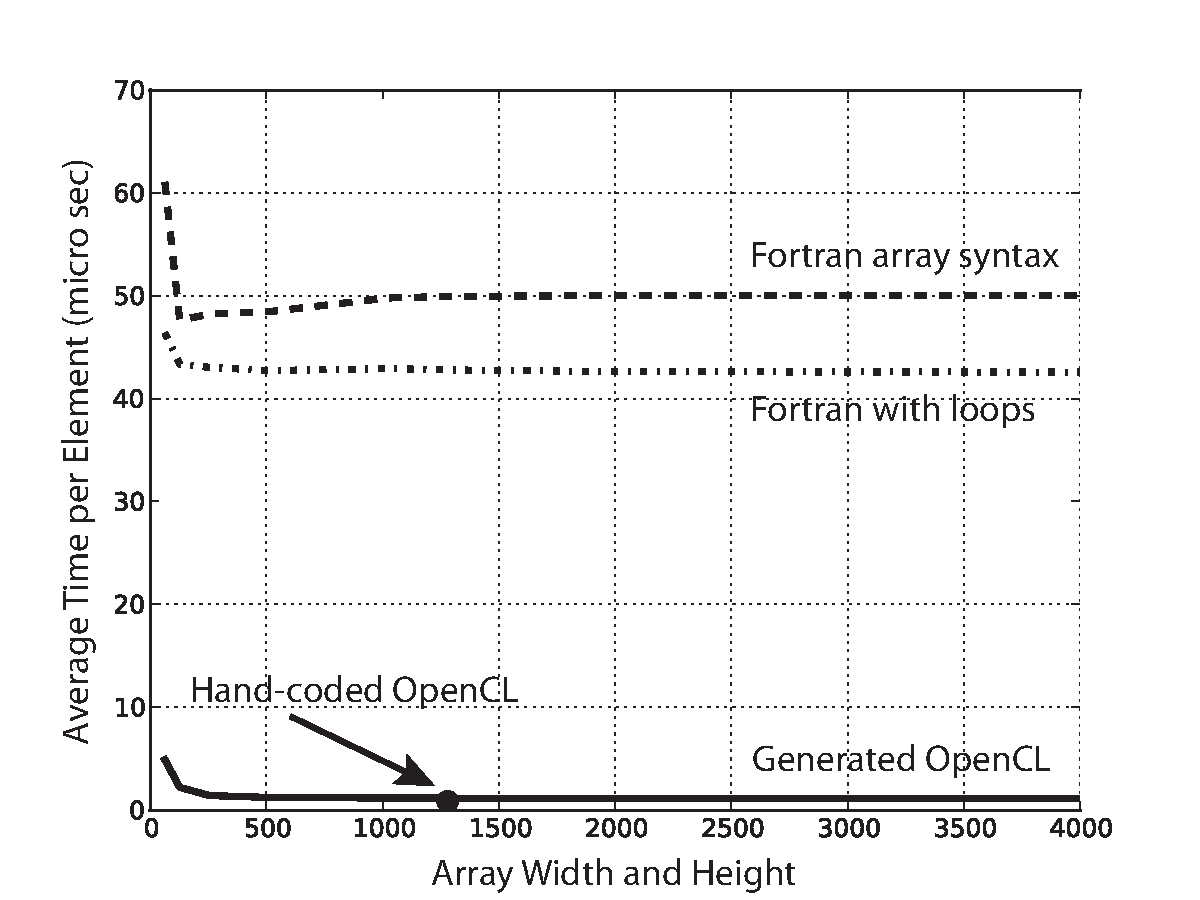
\includegraphics[width=3in]{cl-performance.pdf}
%\caption{Performance comparison for varying array size.}
%\label{fig:cl-performance}
%\end{figure}


\section{Conclusions}

The sheer complexity of programming for clusters of many or multi-core
processors with tens of millions threads of execution make the simplicity of
the data-parallel model attractive.  The increasing complexity of
todays applications (especially in light of the increasing complexity
of the hardware) and the need for portability across architectures
make a higher-level and simpler programming model like data-parallel
attractive.

The goal of this work has been to exploit source-to-source transformations that
allow programmers to develop and maintain programs at a high-level of
abstraction, without coding to a specific hardware architecture.
Furthermore these transformations allow multiple hardware architectures
to be targeted without changing the high-level source.  It also removes the
necessity for application programmers to understand details of the accelerator
architecture or to know OpenCL.

%%TODO \cite{chamberlain04zpl, roth97stencils}

\bibliographystyle{IEEEtran}
\bibliography{IEEEabrv,foropencl}

\end{document}
